\subsection{Vermessung der Spektralinien}
\subsection{Reflexionsgitter}
Mit Hilfe eines Reflexionsgitters werden im Versuch die Wellenlängen von emittiertem Licht bestimmt. Untersucht wird dabei die Lage der Interferenzmaxima des reflektierten Lichtes. Eine wichtige Größe, die das Gitter charakterisiert, ist dabei die Gitterkonstante $d$, die die Periode des Gitters angibt. Mit Hilfe von Abbildung \ref{Gangunterschied} lässt sich leicht der Gangunterschied $g$ zweier benachbarter Strahlen berechnen. Werden die Winkel in mathematisch positiver Richtung zum Lot gemessen erhält man
\begin{align*}
  g=d \cdot (\sin(\alpha)+\sin(\beta)).
\end{align*} 
Für Licht der Wellenlänge $\lambda$ gilt bei den Interferenzmaxima also (mit $n \in \mathbb{Z}$)
\begin{align}
  d \cdot (\sin(\alpha)+\sin(\beta)) = n\lambda.
\end{align}
\begin{figure}[h]
  \centering
  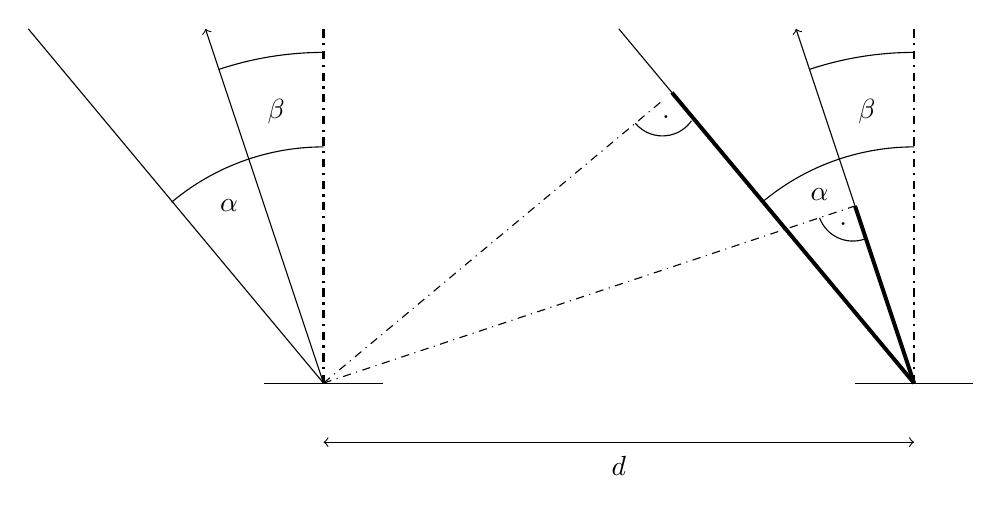
\begin{tikzpicture}[scale=1.5]
    \draw (0,0)--(1,0);
    \draw [thick, dash dot] (0.5,0)--(0.5,3);
    \draw (-2,3)--(0.5,0);
    \draw [->] (0.5,0)--(-0.5,3);
    \draw (0.5,2.8) arc (90:108.5:2.8);
    \draw (0.5,2) arc (90:130:2);
    \draw (0.1,2.3) node {$\beta$};
    \draw (-0.3,1.5) node {$\alpha$};
    \draw (5,0)--(6,0);
    \draw [thick, dash dot] (5.5,0)--(5.5,3);
    \draw (5.5-2.5,3)--(5.5-2.5*0.82,3*0.82);
    \draw [line width=0.5mm] (5.5-2.5*0.82,3*0.82)--(5.5,0);
    \draw [line width=0.5mm] (5.5,0)--(5.5-0.5,0.5*3);
    \draw [->] (5.5-0.5,0.5*3)--(4.5,3);
    \draw (5.5,2.8) arc (90:108.5:2.8);
    \draw (5.5,2) arc (90:130:2);
    \draw (5.1,2.3) node {$\beta$};
    \draw (4.7,1.6) node {$\alpha$};
    \draw [dash dot](0.5,0)--(0.5+2.4*6/5,2.4);
    \draw [dash dot](0.5,0)--(0.5+1.5*3,1.5);
    \draw [<->] (0.5,-0.5)--(5.5,-0.5);
    \draw (3,-0.7) node {$d$};
    \draw (0.5+2.2*6/5,2.2) arc (220:325:0.3);
    \draw (3.4,2.25) node {$.$};
    \draw (0.5+1.4*3,1.4) arc (200:290:0.3);
    \draw (4.9,1.35) node {$.$};
  \end{tikzpicture}
  \caption{Gangunterschied (fett eingezeichnet) für benachbarte Strahlen}
  \label{Gangunterschied}
\end{figure}